% Copyright 2004 by Till Tantau <tantau@users.sourceforge.net>.
%
% In principle, this file can be redistributed and/or modified under
% the terms of the GNU Public License, version 2.
%
% However, this file is supposed to be a template to be modified
% for your own needs. For this reason, if you use this file as a
% template and not specifically distribute it as part of a another
% package/program, I grant the extra permission to freely copy and
% modify this file as you see fit and even to delete this copyright
% notice. 

\documentclass{beamer}
\setbeamertemplate{bibliography item}[text]

% There are many different themes available for Beamer. A comprehensive
% list with examples is given here:
% http://deic.uab.es/~iblanes/beamer_gallery/index_by_theme.html
% You can uncomment the themes below if you would like to use a different
% one:
%\usetheme{AnnArbor}
%\usetheme{Antibes}
%\usetheme{Bergen}
%\usetheme{Berkeley}
%\usetheme{Berlin}
%\usetheme{Boadilla}
%\usetheme{boxes}
%\usetheme{CambridgeUS}
%\usetheme{Copenhagen}
%\usetheme{Darmstadt}
%\usetheme{default}
\usetheme{Frankfurt}
%\usetheme{Goettingen}
%\usetheme{Hannover}
%\usetheme{Ilmenau}
%\usetheme{JuanLesPins}
%\usetheme{Luebeck}
%\usetheme{Madrid}
%\usetheme{Malmoe}
%\usetheme{Marburg}
%\usetheme{Montpellier}
%\usetheme{PaloAlto}
%\usetheme{Pittsburgh}
%\usetheme{Rochester}
%\usetheme{Singapore}
%\usetheme{Szeged}
%\usetheme{Warsaw}

\usepackage{amsmath}
\usepackage[style=verbose,backend=biber]{biblatex}
\addbibresource{\jobname.bib}

\newcommand{\reels}{\mathbb{R}}
\newcommand{\norm}[1]{\left\lVert#1\right\rVert}

\title{Autoencoder is more than a dimensionality reduction tool}

\usepackage{filecontents}
\begin{filecontents}{\jobname.bib}
@TECHREPORT{RePEc:cwl:cwldpp:159,
    title = {A six-factor asset pricing model},
    author = {Rahul Roy, Santhakumar Shijin},
    year = {2018},
    institution = {Borsa Istanbul Review},
    type = {Cowles Foundation Discussion Papers},
    url = {https://hal.archives-ouvertes.fr/hal-01878923/document}
}
\end{filecontents}



\author{Thomas LOUIS}
% - Give the names in the same order as the appear in the paper.
% - Use the \inst{?} command only if the authors have different
%   affiliation.

\date{2019}
% - Either use conference name or its abbreviation.
% - Not really informative to the audience, more for people (including
%   yourself) who are reading the slides online

% Let's get started
\begin{document}

\begin{frame}
  \titlepage
\end{frame}

\begin{frame}[shrink=20]{Outline}
  \tableofcontents
  % You might wish to add the option [pausesections]
\end{frame}

% Section and subsections will appear in the presentation overview
% and table of contents.
\section{Dimensionsionality reduction}

\subsection{Why reducing dimensionality ?}

\begin{frame}{Why reducing dimensionality ?}
    Reducing dimensionality has several industrial applications:
    \begin{itemize}
	    \item coping with dimensionality curse $\rightarrow$  improving algorithm's performance or make them usable
	    \item compressing data $\rightarrow$ saving disk, memory space and processing time 
	    \item denoising data $\rightarrow$ signal processing 
    \end{itemize}
\end{frame}

\subsection{The PCA case}
\begin{frame}{The PCA case}
    Let's $M$ a ${N, d}$ matrix  of N vector $\in \reels^{d}$\\
    M reprents N individuals that present $d$ quantitative variables \\
    We wan't to find iteratively an orthogonal projection base $\mathbf{b}$ for M where the vector projects maximal variance and are ordered by this variance \\
    let $\mathbf{u}$ be the first vector of $\mathbf{b}$ \\
    $\hat{M}$ is the centred, standardized matrix of M \\
    $\hat{M}.\hat{M}^{t}$ is symetric thus diagonalizable : $\hat{M}.\hat{M}^{t} = P^{t}.\Delta.P$ \\
    $u.\hat{M} . (u\hat{M})^{t} = u.\hat{M}.\hat{M}^{t}u{t}$ \\
    $ = u. P^{t}.\Delta.P. u^{t} $

    $\Delta$ contains eigen vectors and P is the projection matrix for its eigenspace \\

    We only keep the eigen vectors that explain the most of the variance of M. \\
\end{frame}

\begin{frame}{The PCA case}
    PCA is able to catpure the linear relationships between correlated variables. \\
    \begin{minipage}{6in}
    \centering
    $\vcenter{
    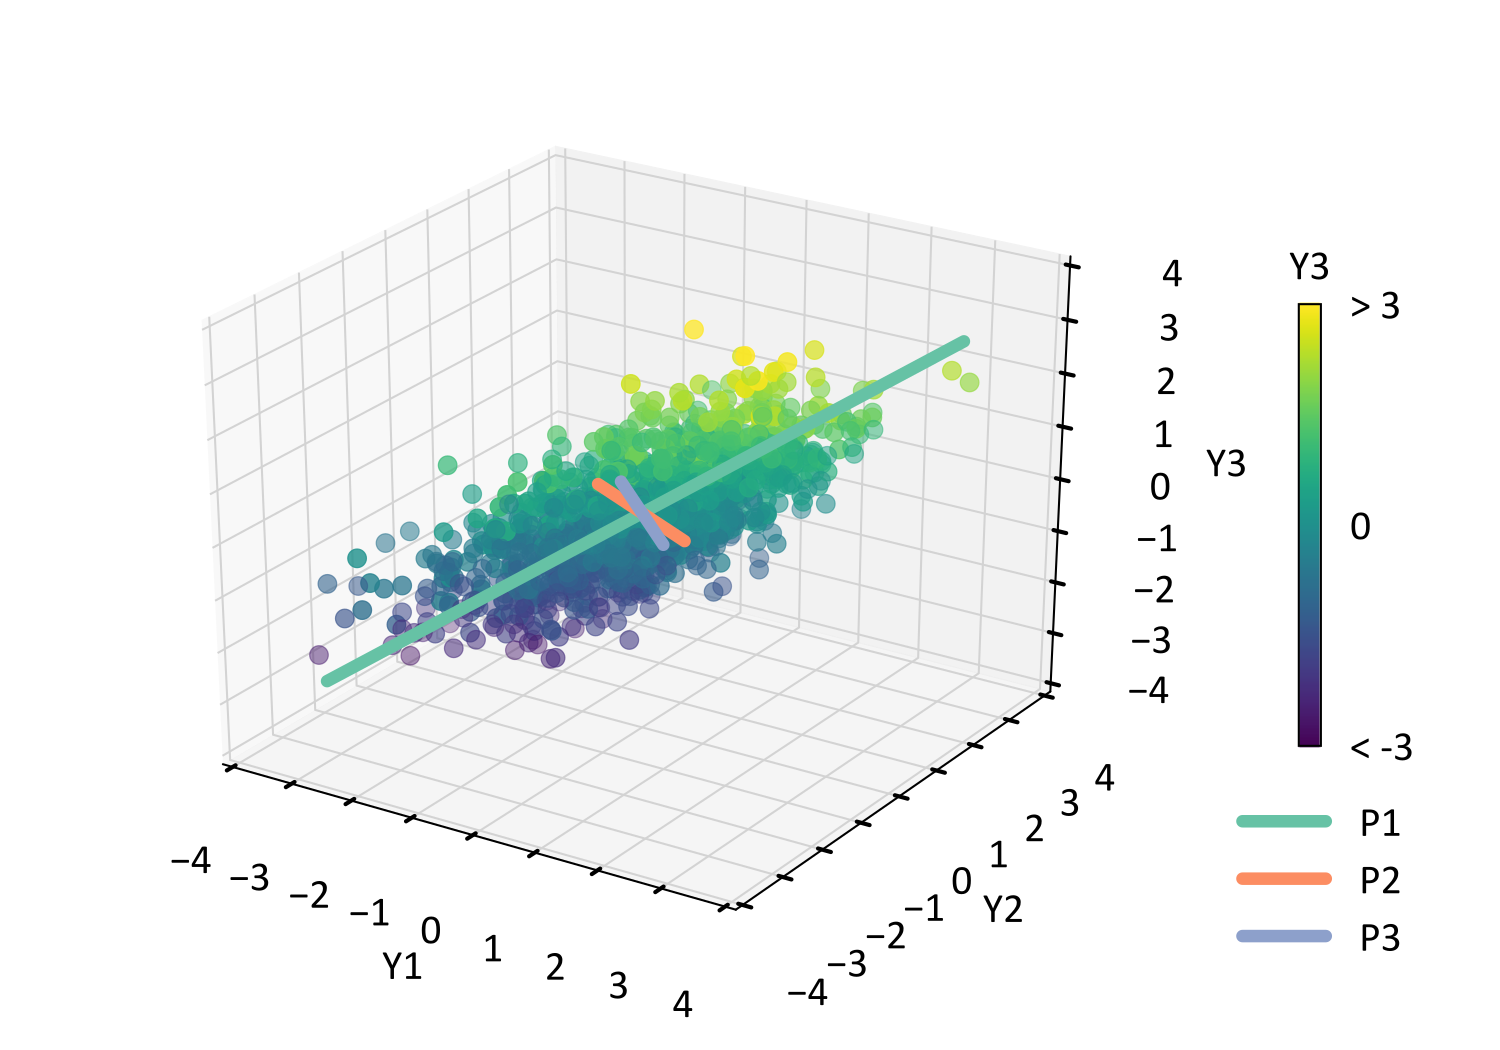
\includegraphics[scale=0.2]{data/pca_3d.png}
    }$
    \end{minipage}
\end{frame}

\begin{frame}{The PCA case}
    example of applications: eigenfaces \\
    \begin{minipage}{6in}
    \centering
    $\vcenter{
    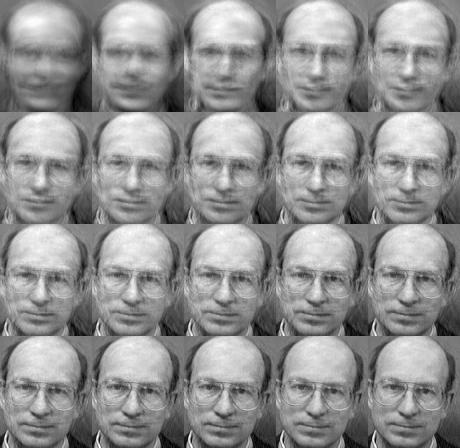
\includegraphics[scale=0.3]{data/eigenfaces.png}
    }$
    \end{minipage}
\end{frame}


\section{Autoencoder}
\subsection{Autoencoder architecture}
\begin{frame}{Autoencoder architecture}
    Autoencoder is a specific neural network meta-architecture composed of:
    \begin{enumerate}
	\item an encoder network $f = \underset{i \in {{1 .. e}}}{O} L_i$
        \item a latent vector $h$ of lower dimension than input dimension 
	\item a decoder network $g = \underset{i \in {{e + 1 .. d + e}}}{O} L_i$
    \end{enumerate}
    With $L_i : x \rightarrow \sigma(W_i.x + b_i)$ \\
    Where the input of the encoder has exactly the same dimensionality as the output of the decoder. \\
    \begin{minipage}{6in}
    \centering
    $\vcenter{
    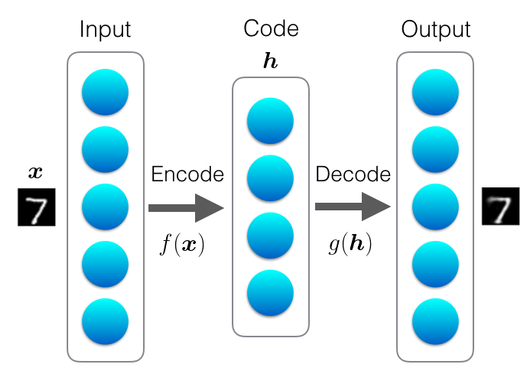
\includegraphics[scale=0.2]{data/autoencoder_illustration.png}
    }$
    \end{minipage}
\end{frame}

\begin{frame}{Autoencoder architecture}
	Being an neural network make it profit from some properties:
	\begin{itemize}
		\item ability to approximate any couple of continuos funcion $(f,g)$ over a compact couple
		\item ability to deal with non linear problems
		\item prediction is done at constant computational cost
		\item ability to optimize different metrics with some assumptions
		\item either supervised or unsupervised approach
	\end{itemize}
	autoencoder are meta-architecture that can compose with neural network to specialize to data
	\begin{itemize}
		\item CNN, ResNet for images 
		\item RNN for sequential data
		\item GCN for graphs
	\end{itemize}
\end{frame}

\subsection{Autoencoder optimization}
\begin{frame}{Autoencoder optimization}
	\begin{itemize}
		\item The output must reconstruct the input while having a bottleneck
		\item $(W_i)_{i \in {1 .. e+d}} = \underset{(W_i)_{i \in {1 .. e+d}}}{argmin} \norm{ x - g \circ f(x)}_f$
		\item Optimization is done using backpropagation algorithm
	\end{itemize}
\end{frame}

\subsection{Similarities with PCA}
\begin{frame}{Similarities with PCA}
	A linear autoencoder with one hidden layer is close to PCA\\
	We can rewrite $g \circ f (x)$ as $A.B.x$ or $C.x$ with $C = A.B$\\
	then we want to optimize $\norm{ M - C.M)}_f$ \\ 
	if $B = A^{t}$ we have $\norm{A^{t}.A - Y}_f = \norm{ P^t \Delta P. X - X}_f => ... $
\end{frame}

\begin{frame}{Similarities with PCA}
    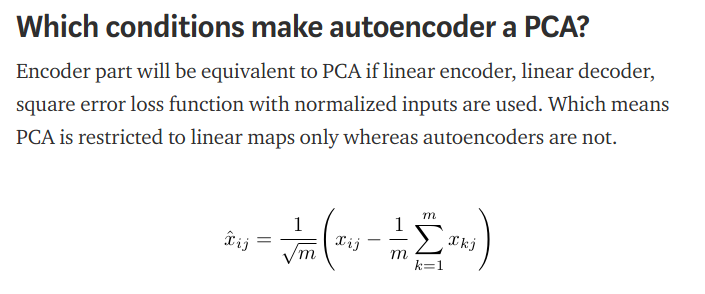
\includegraphics[scale=0.4]{data/pca_vs_autoencoder_bullshit1.png}
\end{frame}

\begin{frame}{Similarities with PCA}
    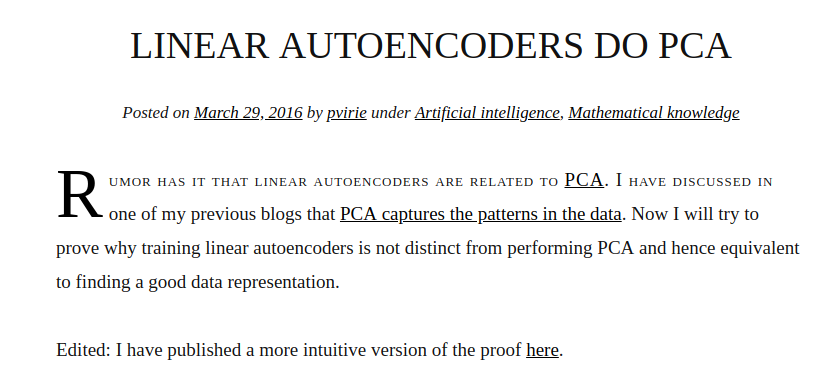
\includegraphics[scale=0.4]{data/pca_vs_autoencoder_bullshit2.png}
\end{frame}

\begin{frame}{Similarities with PCA}
	\begin{itemize}
		\item PCA : M' = S.M  
		\item AE : H = A.X
	\end{itemize}
We have close minimization objectives but orthogonality of $h$ is never ensured.
\end{frame}


\subsection{Transforming a linear autoencoder into a PCA solver}
\begin{frame}{Transforming a linear autoencoder into a PCA solver}
	Let's optimize $E = \norm{ X - W_g.(W_f.X + b_f) + b_g.u^{t}}$
	Transforming a one hidden layer linear autoencoder into a PCA solving E = 0: \\
	If we force $\underset{b_g}\nabla  \norm{ X - W_g.(W_f.X + b_f) + b_g.u^{t}}_f$ to 0
	Then: \\
	as $\norm{A}_{f} = tr(A^{t}.A)$  we have $b_{g} = 1/N * (X - W_{g}.H).u $ \\
	$E = \norm{X^{'} - W_{g}.H^{'}}$ with $X' = X(I - u.u^{t}/N)$ and $H' = H(I - u.u^{t}/N)$ \\
\end{frame}
\begin{frame}{Transforming a linear autoencoder into a PCA solver}
	we consider SVD of $X^{'} = U_x\Sigma_{x}V_x^{t}$ and $W_g.H^{'} = U_w.\Sigma_{w}.V_w^{t}$ \\
	$W_g = U_w.T^{-1}$ and $H^{'} = T.\Sigma_w.V_w^{t}$ \\
	$C_x = X'(X^{'})^{t} = U_x.(\Sigma_x)^{2}.U_x^{t}$ \\
	$C_w = W_g.H'(W_g.H^{'})^{t} = U_w.(\Sigma_w)^{2}.U_w^{t}$ \\
	$W_{f}X = H \rightarrow W_{f}X^{'} = b_{w}.u^{t}(I - u.u^{t}/N)$ \\
	$W_{f} = T.(U_{w})^{t}$ \\
	Thus for arbitrary $b_{f}$ we have $b_{g} = (I - U_{w}.(U_{w})^{t})\mu_X - U_{w}.T^{-1}.b_{f}$
\end{frame}


\section{Using autoencoder for pricing}
\subsection{Asset returns model}
\begin{frame}{Asset returns model}
	A common model for asset return is a linear K-factor model : \\
	$r_{i,t} = (\beta z_{i,t - 1})^{t}.f_t + u_{i,t}$ \\
    $R = \beta^t.F + U$
	where $\beta$ is a function over asset caracteristics high dimensional vector $z_i$ of size $(L, 1)$, at time t-1.
	$f_t$ is a latent vector. $u_{i,t}$ is an idiosyncratic error vector. \\
	Find $\beta$, $f_t$, that fit the model.
\end{frame}

\subsection{PCA view}
\begin{frame}{Asset returns model}
    Let's define our autoencoder architecture iteratively: \\
    for each layer $l$ we have the output $r^{l}$ : \\
    $r^{l} = g(b^{l-1} + r^{l-1}.W^{l-1})$
    we want to optimize the parameter for the loss $L$.
    $\hat{W},\hat{b} = \underset{W,b}{argmin} \underset{i=1..T}{\Sigma} \norm{r_t - (b^{1} + W^{1}.(b^{0} + W^{0}. r_t))}$ \\
    For a 1 hidden layer autoencoder, with identity as activation function. one optimal solution is the solution of a PCA. \\
    \begin{itemize}
	    \item $\hat{W}^{(1)} = P.A$ where P is defined by $R = P.\Lambda.Q + U$ and A is a non-singular matrix \\
	    \item $\hat{W}^{(0)} = (\hat{W}^{(1)}^{T}.\hat{W}^{(1)})^{-1}.\hat{W}^{(1)}^t$ \\
	    \item $\hat{b}^{(1)} = R - (\hat{W}^{(1)}.\hat{b}^{(0)} - \hat{W}^{(1)}).\hat{W}^{(0)}.R$ \\
	    \item $\hat{b}^{(0)} = c$, c is a constant
    \end{itemize}
\end{frame}


\subsection{Adding covariates}
\begin{frame}{Asset returns model}
    We want to create both latent vectors and add covariates
    \begin{minipage}{5in}
    \centering
    $\vcenter{
    \includegraphics[scale=0.3]{data/ConditionalAE.png} \\
    }$
    \end{minipage}
\end{frame}

\section{Variational Autoencoder}
\subsection{A Bayesian point of view}
\begin{frame}{Variational Autoencoder - A Bayesian point of view}
    We not only want to map one element to it's simbling with reduced representation.
    We want to learn distribution of the data $\mathbf{p(X)}$ \\
    $ \mathbf{p(x)} = \int_\Omega p(x|t)p(t) dt$  \\
	With assumption over the prior: $p(t) = \mathcal{N}(0, I)$ \\
	$ p(x| t) = \mathcal{N}(\mu(t),\,\Sigma(t))$ \\
	\begin{itemize}
		\item $ \mu(t) = NN_1(t)$
		\item $ \Sigma(t) = NN_2(t)$
	\end{itemize}
	We want to compute $\underset{\omega}{argmax} p(x| \omega) = \int_\Omega p(x|t, \omega)p(t) dt$  \\
\end{frame}

\begin{frame}{Variational Autoencoder - A Bayesian point of view}
	$\underset{\omega}{argmax} p(X|t, \omega) = \underset{\omega}{argmax} log(p(X| \omega))$ \\
	$ log(p(X| \omega)) = \underset{i \in \{1..N\}}{\Sigma} log( \int_\Omega p(x_i, t | \omega))dt$ \\ 
	$ >= \underset{i \in \{1..N\}}{\Sigma} \int_\Omega q(t) log( p(x_i, t | \omega)/q(t))dt$ using Jensen inequality as log is concave\\
	$ = ELOB(w)$ \\
\end{frame}
\begin{frame}{Variational Autoencoder - A Bayesian point of view}
	$ = \underset{i \in \{1..N\}}{\Sigma} \int_\Omega q(t) log( p(x_i | \omega, t).p(t)/q(t))dt$ \\
	$ = \underset{i \in \{1..N\}}{\Sigma} \int_\Omega q(t) log( p(x_i | \omega, t))dt + \int_\Omega q(t)log(q(t)/p(t)) dt$ \\
	$ = \underset{i \in \{1..N\}}{\Sigma} \int_\Omega q(t) log( p(x_i | \omega, t))dt + KL( q || p) $ \\
	$ log(p(X|t, \omega)) >= ELOB(\omega,q) $
	We have a reconstruction loss term plus a KL divergence term
\end{frame}

\begin{frame}{Variational Autoencoder - A Bayesian point of view}
	$ \underset{\omega}{argmax} p(X|t, \omega) >= L(\omega,q) $ \\
        $ \underset{\omega,q}{argmax} L(\omega,q) $ \\
	each object $x_i$ has its own variational distribution $q_i$ \\
        $ \underset{\omega,q}{argmax} L(\omega,q_1, q_2, ... q_N) $ \\
	We'll approximate each $q_i$ with a Gaussian distribution $q_i = \mathcal{N}(m_i,\,\sigma_i)$ \\
	We use here the encoder to compute the latent distribution: \\
	\begin{itemize}
		\item $m_i = m(x_i, \phi)$
		\item $\sigma_i = \sigma(x_i, \phi)$
	\end{itemize}
	Thus $\phi$ is our encoder that from the input, compute the corresponding latent value.
\end{frame}

\begin{frame}{Variational Autoencoder - A Bayesian point of view}
    \begin{minipage}{5in}
    \centering
    $\vcenter{
    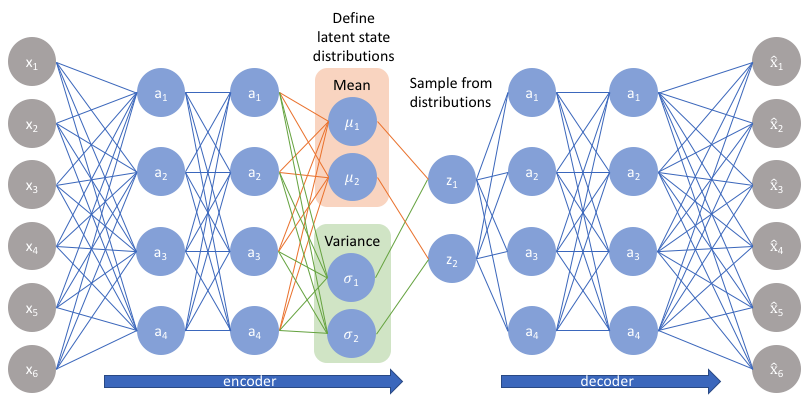
\includegraphics[scale=0.3]{data/variational_autoencoder.png} \\
    }$
    \end{minipage}
    $ L(\omega, \phi, X)= \underset{i \in \{1..N\}}{\Sigma} \int_\Omega q_\phi(t) log( p(x_i | \omega, t) dt) + KL( q || p ) $
\end{frame}


\subsection{Optimization}
\begin{frame}{Variational Autoencoder - Optimization}
        $ L(\omega, \phi, X)= \underset{i \in \{1..N\}}{\Sigma} \int_\Omega q_\phi(t) log( p(x_i | \omega, t) dt) + KL( q_\phi || p ) $\\
	We now need to compute $\nabla L(\omega, \phi).$.\\
	Experimentaly, this preforms poorly due to logartihm of probabilities that are very low at the beginning\\
	What we do instead is to compute $\underset{\phi}{\nabla} L(\omega,\phi)$, by sampling $t_i$ \\
	$t_i = m_i + \sigma_i * \epsilon_i$ \\
	In order to be able to compute back propagation, we sample $\epsilon_i$ from  $\mathcal{N}(0,I)$
\end{frame}

\begin{frame}{Variational Autoencoder - Optimization}
    \begin{minipage}{5in}
    \centering
    $\vcenter{
    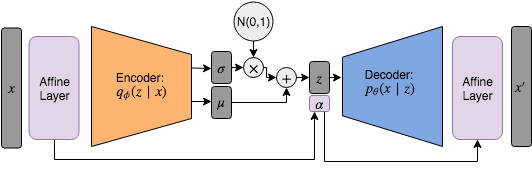
\includegraphics[scale=0.5]{data/variational_autoencoder_reparametrized.png} \\
    }$
    \end{minipage}
\end{frame}

\section{Disentangled Variational Autoencoder}
\subsection{Disentangling lattent representations}
\begin{frame}{Disentangling lattent representations}
	Vanilla VAE isn't sufficient:
	\begin{itemize}
		\item No insurrance about how meaningfull/relevant latent space is 
		\item No insurrance about how the autoencoder can generalize over new data 
	\end{itemize}
    \bf{Disentangled Variational Autoencoder}
	$ L(\omega, \phi, X)= \underset{i \in \{1..N\}}{\Sigma} \mathbb{E}_{q_\phi(t_i)} log( p(x_i | \omega, t_i)) + \beta KL( q_\phi || p ) $
\end{frame}

\begin{frame}{Disentangling lattent representations}
    \begin{minipage}{5in}
    \centering
    $\vcenter{
    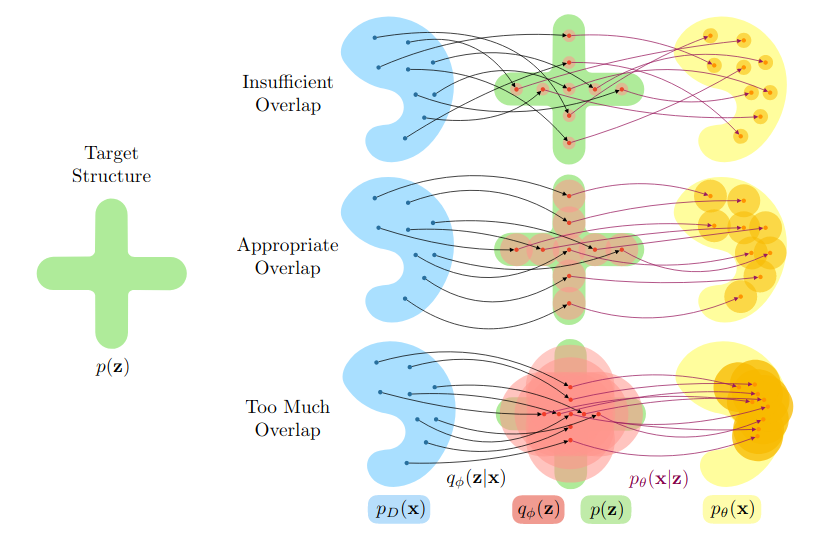
\includegraphics[scale=0.4]{data/disentanglement.png} \\
    }$
    \end{minipage}
\end{frame}


\begin{frame}{Disentangling lattent representations}
    A very important experimental result: \\
    \begin{minipage}{5in}
    \centering
    $\vcenter{
    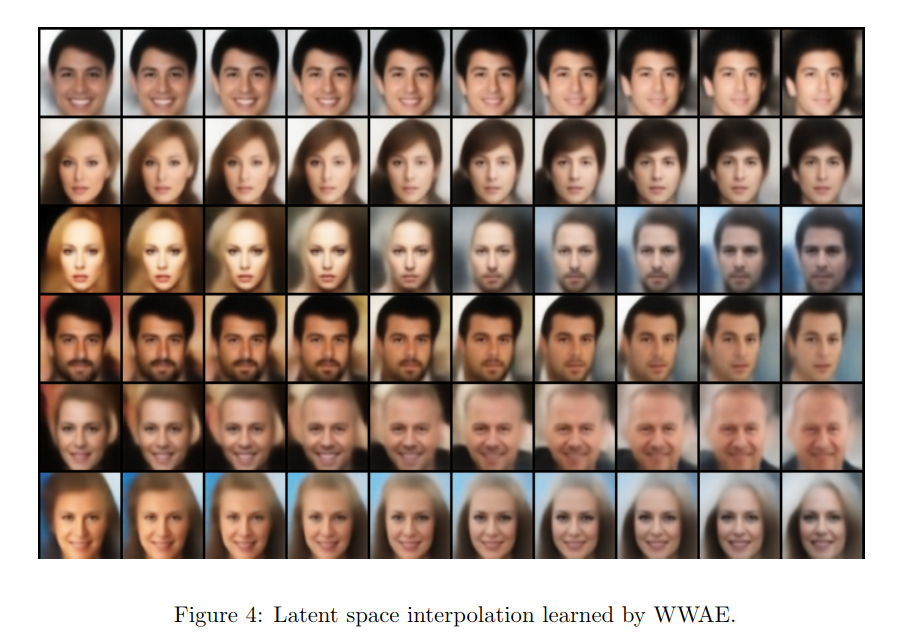
\includegraphics[scale=0.3]{data/wwae.png} \\
    }$
    \end{minipage}
    linear combination of two latent variable as a decoder image included in the space of the target 
\end{frame}


\subsection{VAE Applications}
\begin{frame}{VAE Applications}
    We don't really have p(x), but it is learned into the VAE.\\
    What if the reconstruction error expoldes when we set $x_0$ as input of the encoder ? \\
    We've just spotted an anomaly !!!
    This is a really widely used strategy for anomaly detection with many applications:
    \begin{itemize}
        \item e-transaction fraud detection
        \item anomaly market
        \item price anomaly
	\item beyond entropy compression
	\item segmentation
    \end{itemize}
\end{frame} 

\section{How to use an Autoencoder ?}
\begin{frame}{How to use an Autoencoder ?}
    Just create a model with many neurons and fit it to the data
\end{frame}

\begin{frame}{How to use an Autoencoder ?}
    Just create a model with many neurons and fit it to the data ...
\end{frame}

\begin{frame}{How to use an Autoencoder ?}
    Just create a model with many neurons and fit it to the data ... NO
\end{frame}

\begin{frame}{How to use an Autoencoder ?}
    Problems:
    \begin{itemize}
        \item High Dimensionaity Curse
        \item Hyperparameter sensitivity 
        \item Black boxes 
    \end{itemize}
\end{frame}

\begin{frame}{How to use an Autoencoder ?}
    Solutions:
    \begin{itemize}
        \item High Dimensionaity Curse $\rightarrow$ break dimensionality with your human prior
        \item Hyperparameter sensitivity $\rightarrow$ Optimization and rule of thumb 
        \item Black boxes $\rightarrow$ Validate your model with model explaination
    \end{itemize}
\end{frame}

\begin{frame}{Examples}
    \begin{minipage}{5in}
    \centering
    $\vcenter{
    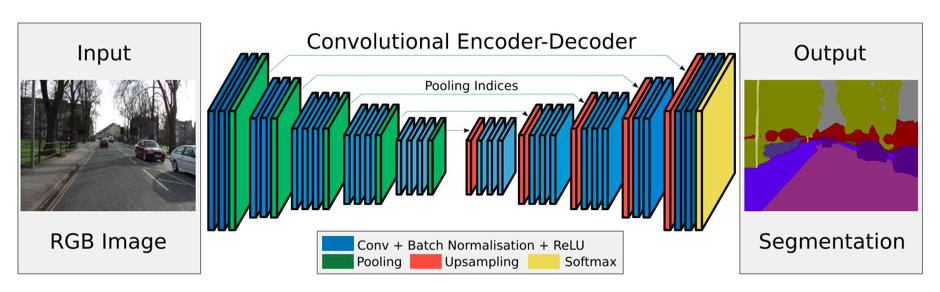
\includegraphics[scale=0.3]{data/cnn_autoencoder.png} \\
    }$
    \end{minipage}
\end{frame}

\section{Conclusion}
\begin{frame}{Conclusion}
    Autoencoders are powerfull tools to reduce data dimension and retain meaningfull information from dataset.
    They became state of the art model and model component for many applications in many industries including finance.
\end{frame}

\section{To go further}
\begin{frame}{To go further}
\begin{itemize}
        \item Generative Adversarial Network
        \item Lattent embedding sharing
        \item Consciouness
\end{itemize}
\end{frame}

\end{document}


